\chapter{Requirements of a Runtime Configuration System (RCS)}
\label{chapter:requirements}

To be able to assess how suitable existing related work is, or if it is necessary to design a completely new architecture to fulfill the requirements for runtime configuration inside \gls{gl:riot_os}, it is first necessary to define what is needed and why.

\section{Shared \acrlongpl*{ac:cs}}
\label{sec:requirements:shared_pre_defined_configuraiton_schemas}

A \glsfirst{ac:cs} is mostly a data structure combined with some additional metadata such as parameter types or preconditions.
For a \gls{gl:configuration_manager} to be easily integrated into other external tools, it is necessary to have a collection of \glspl{ac:cs} to describe common configuration needs.
For example, there could be an LED \gls{ac:cs} consisting of three unsigned 8-bit integer variables, or a WI-FI \gls{ac:cs} containing the SSID, the password, etc.
Now, these \glspl{ac:cs} are supposed to be implemented by for example LED drivers, or WI-FI module drivers.
This way the registry has a consistent \gls{ac:api}, as can be seen on the right-hand side of \autoref{fig:evaluation:requirements:shared_pre_defined_configuraiton_schemas}.

An alternative approach is to define a custom \gls{ac:cs} per module basis, as can be seen on the left-hand side of \autoref{fig:evaluation:requirements:shared_pre_defined_configuraiton_schemas}.
This results in a lot of duplicated work and inconsistent \glspl{ac:api} for equal operations.
The advantage of this approach is that the work put into defining the custom \gls{ac:cs} is less than specifying a \gls{ac:cs} that has to fit for all comparable use-cases.
So new modules/driver that require a certain configuration module that is for example not yet implemented in the registry would just specify their own and don't need to find a solution for all first.
This would save a lot of review time and helps adoption.

If each approach's advantages and disadvantages are compared, having a consistent \gls{ac:api} outweighs the time saving of a per-module approach and is worth spending some extra time for, as this extra work is not wasted, but essential to enable the integration of external \glspl{gl:configuration_manager}. With no consistent \gls{ac:api}, those tools would need to be adapted to every single driver instead of just the \glspl{ac:cs}, that are shared among modules.

\begin{figure}[H]
    \centering
    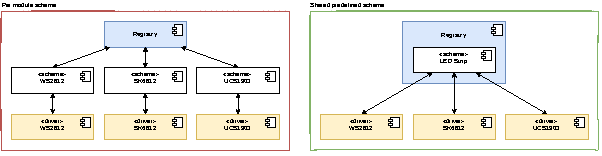
\includegraphics[width=\textwidth]{requirements_shared_pre_defined_configuration_schemas}
    \caption{Per module \glspl{ac:cs} (left-hand side) and Shared \glspl{ac:cs} (right-hand side).}
    \label{fig:evaluation:requirements:shared_pre_defined_configuraiton_schemas}
\end{figure}

\section{Multiple Instances per \acrlong*{ac:cs}}
\label{sec:requirements:multiple_instances_per_schema}

This requirement is strongly connected to \autoref{sec:requirements:shared_pre_defined_configuraiton_schemas}.
Having shared \glspl{ac:cs} requires that these can be used at the same time, by multiple modules, as can be seen on the right-hand side of \autoref{fig:evaluation:requirements:multiple_instances_per_schema}, without causing conflicts as can be seen on the left-hand side of \autoref{fig:evaluation:requirements:multiple_instances_per_schema}.
If an example application has 3 different LED modules, of which each implements the same LED \gls{ac:cs}, they need to expose their data in their instance of this \gls{ac:cs} and don't overwrite each other's configurations.
Besides that even if there is only one module, that is used to control three LEDs of the same kind, it is also necessary for this module to create multiple instances so that each LED can be configured on its own.

This means that the \gls{ac:cs} should not hold the actual data but only specify its structure.
Modules then shall be able to create as many instances of this \gls{ac:cs} as is needed.

\begin{figure}[H]
    \centering
    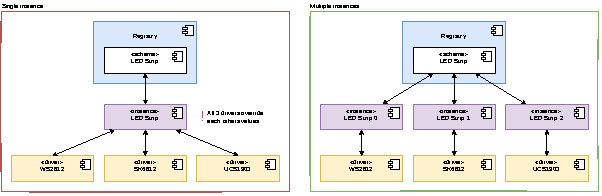
\includegraphics[width=\textwidth]{requirements_multiple_instances_per_schema}
    \caption{Single shared instance (left-hand side) and Multiple instances (right-hand side).}
    \label{fig:evaluation:requirements:multiple_instances_per_schema}
\end{figure}

\section{Integer Path as the Identifier of Configuration Values}
\label{sec:requirements:integer_path_as_identifier_of_configuration_values}

To uniquely identify each configuration parameter a path or array is needed that points to the parameter.
For example ``schema\_id/instance\_id/parameter\_id''.

One way to do this is using an array of strings, as can be seen on the left-hand side of \autoref{fig:evaluation:requirements:integer_path_as_identifier_of_configuration_values}, inspired by the URI in HTTP \cite{RFC-3986}.
This approach is very verbose, which is good for integrations such as \gls{gl:mqtt} \cite{mqtt311} or \gls{ac:coap}, which also rely on using string based identifier paths.
It is also significantly less difficult for humans to work with compared to numbers for example.
The downside of using strings is a huge amount of overhead, especially for constrained devices.
Not only in terms of processing power that is necessary to path strings compared to simple arrays of numbers, but most importantly in terms of unnecessary payload when accessed remotely.
For example through LoRA, which in some scenarios could make every single byte count \cite{avtms-ull-17}.

Using integers instead of strings does not come with these issues, but also has some disadvantages, such as a lower human readability, as can be seen on the right-hand side of \autoref{fig:evaluation:requirements:integer_path_as_identifier_of_configuration_values}.
But \gls{gl:riot_os} is an operating system for constrained devices and this is why low connectivity and low power scenarios are more important use-cases than human readability.
Also, if the parameter identifier is based on an integer path, it is possible to give parameters optional string identifiers to improve the integration of external tools and also improve human readability.
(Besides that modern IoT configuration protocols such as the \gls{ac:coap} Management Interface (CORECONF) \cite{draft-ietf-core-comi-11} also use integers as identifiers, which does not mean it is the right to choose in this case, but still strengthens the point.)

As a conclusion, integer arrays with optional string metadata fields are a solid solution for runtime configuration parameter identifiers of constrained devices.

\begin{figure}[H]
    \centering
    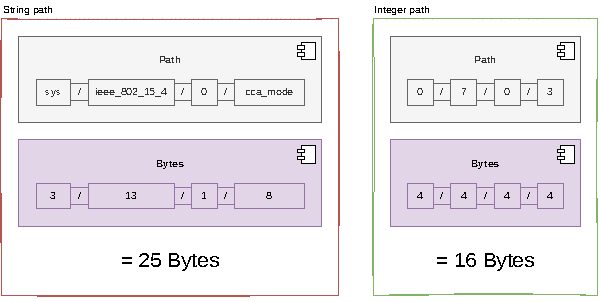
\includegraphics[width=\textwidth]{requirements_integer_path_as_identifier_of_configuration_values}
    \caption{String path (left-hand side) and Integer path (right-hand side).}
    \label{fig:evaluation:requirements:integer_path_as_identifier_of_configuration_values}
\end{figure}

\section{Nested \acrlongpl*{ac:cg}}
\label{sec:requirements:nested_configuration_groups}

A \gls{ac:cs} can either have a nested file system like structure of \glspl{ac:cg} (folders) that contain parameters (files) or even more \glspl{ac:cg} as can be seen on the right-hand side of \autoref{fig:evaluation:requirements:nested_configuration_groups}, or on the other hand, it can also be implemented just as a flat key-value structure as can be seen on the left-hand side of \autoref{fig:evaluation:requirements:nested_configuration_groups}.

From the implementation perspective, a key-value structure is less difficult to implement, but it gives the \gls{ac:cs} less flexibility and could cause workarounds such as long parameter name tags. For example ``group1\_group2\_group3\_parameter0'' or ``group2\_group9\_group7\_parameter5''.

As a conclusion, to give more flexibility it is preferred to have the ability to specify nested configuration structures, but it is not an important requirement and does not decide whether a possible implementation is suitable or not.

\begin{figure}[H]
    \centering
    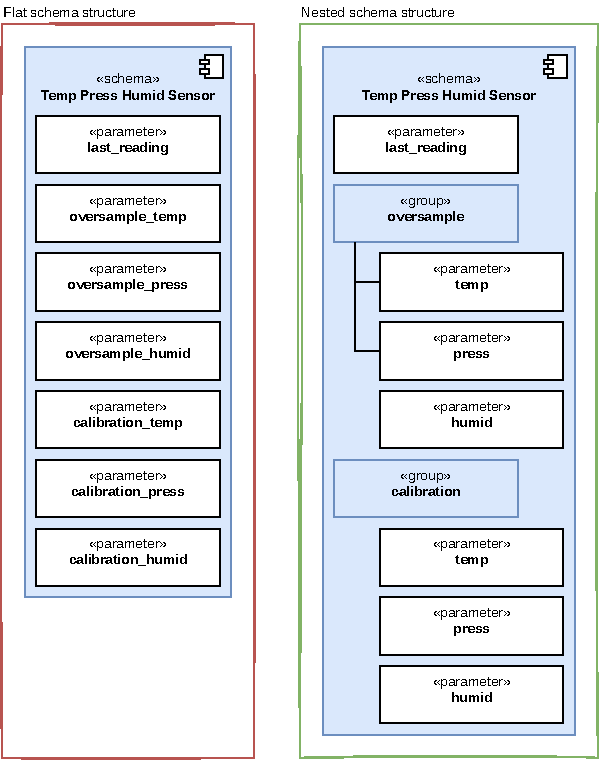
\includegraphics[width=\textwidth]{requirements_nested_configuration_groups}
    \caption{Flat schema structure (left-hand side) and Nested schema structure (right-hand side)}
    \label{fig:evaluation:requirements:nested_configuration_groups}
\end{figure}

\section{Typed Configuration Parameters}
\label{sec:requirements:typed_configuration_parameters}

The types of configuration parameters must be exposed as can be seen on the right-hand side of \autoref{fig:evaluation:requirements:typed_configuration_parameters}.
This allows defining typed external \glspl{ac:api}.

If the type of a configuration parameter is not exposed as can be seen in \autoref{fig:evaluation:requirements:typed_configuration_parameters}, it can not be passed on to external \glspl{ac:api}, allowing errors to occur caused by incompatible input data.

\begin{figure}[H]
    \centering
    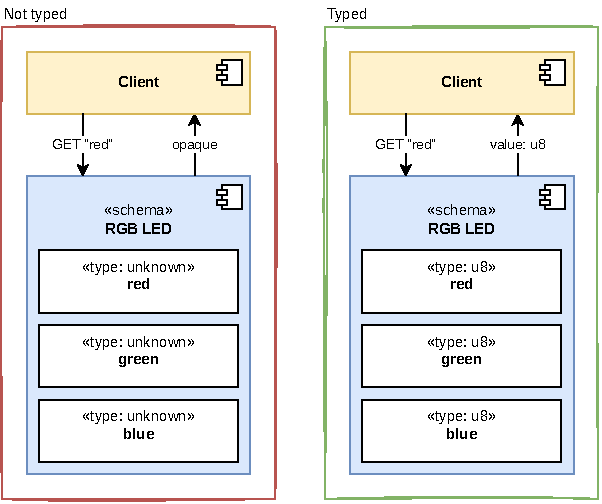
\includegraphics[width=\textwidth]{requirements_typed_configuraton_parameters}
    \caption{Not typed parameters (left-hand side) and Typed parameters (right-hand side).}
    \label{fig:evaluation:requirements:typed_configuration_parameters}
\end{figure}

\section{Binary Internal Configuration Parameter Value Format}
\label{sec:requirements:binary_internal_configuration_parameter_format}

Internally the values of the configuration parameters should be stored and passed around in their binary representation (their correct c type) as can be seen on the right-hand side of \autoref{fig:evaluation:requirements:binary_internal_configuration_parameter_format} and not converted to some inefficient format such as a string as can be seen on the left-hand side of \autoref{fig:evaluation:requirements:binary_internal_configuration_parameter_format}.

The reason for this is that strings have the following drawbacks that are especially problematic with constrained devices:

\begin{enumerate}
    \item In most cases strings consume significantly more storage than the corresponding types needed to represent the same data.

    \item Additionally, heap allocation should be avoided on constrained devices as their storage is usually small and if a program can run or not is best to be known by making sure if the binary fits on the storage or not.
          So to work with string values internally implies always storing the maximum allowed string length for each parameter, to avoid dynamic heap allocation.
          This causes an unnecessarily high amount of storage and possibly stack overhead.
          By using the concrete types, the size of each parameter is always exactly known and is never too large.

    \item Converting from- and to a string, or comparing strings causes a lot of computing overhead that can be avoided.
\end{enumerate}

\begin{figure}[H]
    \centering
    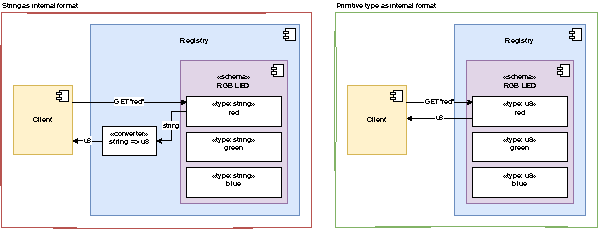
\includegraphics[width=\textwidth]{requirements_binary_internal_configuration_parameter_format}
    \caption{``String as an internal format'' (left-hand side) and Primitive type as an internal format (right-hand side).}
    \label{fig:evaluation:requirements:binary_internal_configuration_parameter_format}
\end{figure}


\section{Transactionally Commit Configuration Changes}
\label{sec:requirements:transactionally_commit_configuration_changes}

In some situations it is necessary that multiple configuration parameters change their value at the same time.
For example these configuration parameters depend on each other, such as an RGB LED that has three configuration parameters, one for red, one for green and one for blue.
If these parameters don't all change at the same time, the color of the RGB LED will not go from for example red to blue, but from red to black and then to blue or from red to pink and then to blue.
So the \gls{ac:rcs} must have the ability to fulfill this need by committing multiple configuration parameter changes in a transactional way.

\section{Persistent Configurations}
\label{sec:requirements:persistent_configurations}

Once a configuration parameter's value is changed, it muste be possible to persist this change on a non-volatile storage.
This is important because especially constrained \gls{ac:iot} devices can have power losses, for example if they are operated by solar energy.

\section{Low Implementation Effort for Modules/Drivers}
\label{sec:requirements:low_implementation_effort_for_modules_and_drivers}

The implementation effort that is necessary to get the \gls{ac:rcs} integrated into each module must be as low as possible while still fulfilling all requirements defined in this section.

If the implementation cost becomes too high, this not only makes maintainability of modules/drivers harder but lowers the chance of high adoption of this runtime configuration module into other drivers/modules in the first place.

\section{Integration with External \glspl*{gl:configuration_manager}}
\label{sec:requirements:integration_with_external_configuration_managers}

The \gls{ac:rcs} must be compatible with common external \glspl{gl:configuration_manager}.
The runtime configuration module is not supposed to specify how external configuration management works for example by introducing an official \gls{ac:coap} \gls{ac:api} but is thought of as an internal \gls{ac:api} that can be used by external \gls{gl:configuration_manager} modules that then expose this \gls{ac:api} however needed.

Currently planned external \gls{gl:configuration_manager} integrations, to which this internal
runtime configuration module must be compatible to are:

\begin{itemize}
    \item A \gls{gl:lwm2m} server \cite{oma-lwm2m-core-12}
    \item A custom \gls{ac:coap} based \gls{ac:api} \cite{RFC-7252}
    \item A custom \gls{gl:mqtt} based \gls{ac:api} \cite{mqtt311}
\end{itemize}
